
\includegraphics[height=1.25cm]{images/pictograms/replication}

\includegraphics[height=1.25cm]{images/pictograms/benchmark}

\includegraphics[height=1.25cm]{images/pictograms/triangle}

\includegraphics[height=1.25cm]{images/pictograms/FEM}

\includegraphics[height=1.25cm]{images/pictograms/paraview}

%%%%%%%%%%%%%%%%%%%%%%%%%%%%%%%%%%%%%%%%%%%%%%%%%%%%%%%%%%%%%%%%%%%%%%%%%%%%%%%%%%%%%%%%%%%%%%%%%%%

\begin{flushright} {\tiny {\color{gray} python\_codes/fieldstone\_46/text.tex}} \end{flushright}

%\lstinputlisting[language=bash,basicstyle=\small]{python_codes/template_keywords.key}

\par\noindent\rule{\textwidth}{0.4pt}

\begin{center}
\inpython
{\small Code: \url{https://github.com/cedrict/fieldstone/tree/master/python_codes/fieldstone_46}}
\end{center}

\par\noindent\rule{\textwidth}{0.4pt}
%%%%%%%%%%%%%%%%%%%%%%%%%%%%%%%%%%%%%%%%%%%%%%%%%%%%%%%%%%%%%%%%%%%%%%%%%%%%%%%%%%%%%%%%%%%%%

This \stone showcases the Crouzeix-Raviart element (see Section~\ref{MMM-sec:crouzeix-raviart})
used to solve the analytical problem "Donea \& Huerta" (see Section~\ref{MMM-mms1}).

Note that the assembled matrices $\K$ and $\G$ are first built and then assembled
into the Stokes matrix, all not in sparse format. As such the code is not very efficient 
and memory requirements increase quickly. 

\begin{center}
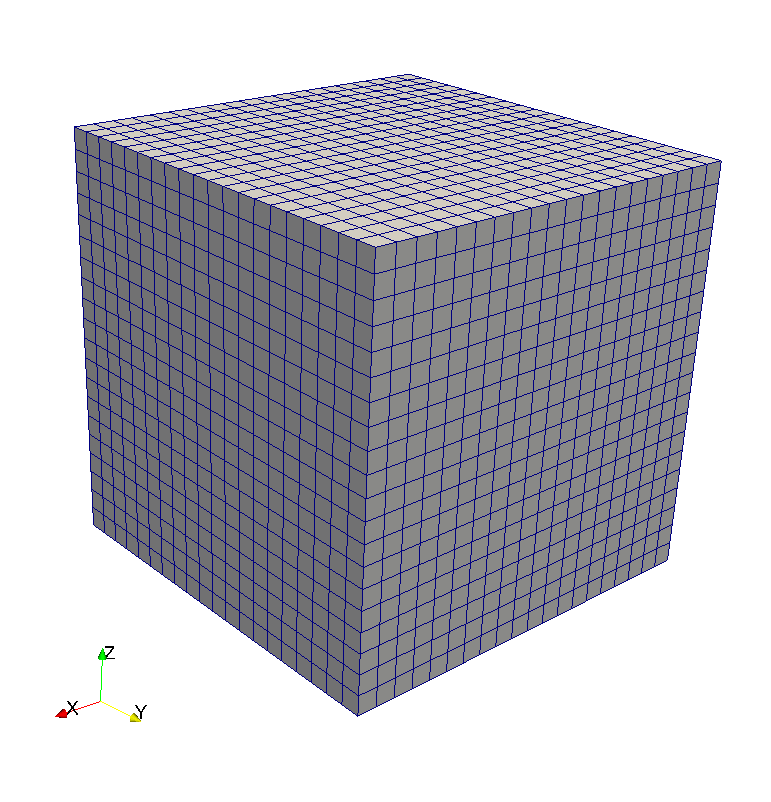
\includegraphics[width=5cm]{python_codes/fieldstone_46/results/grid}
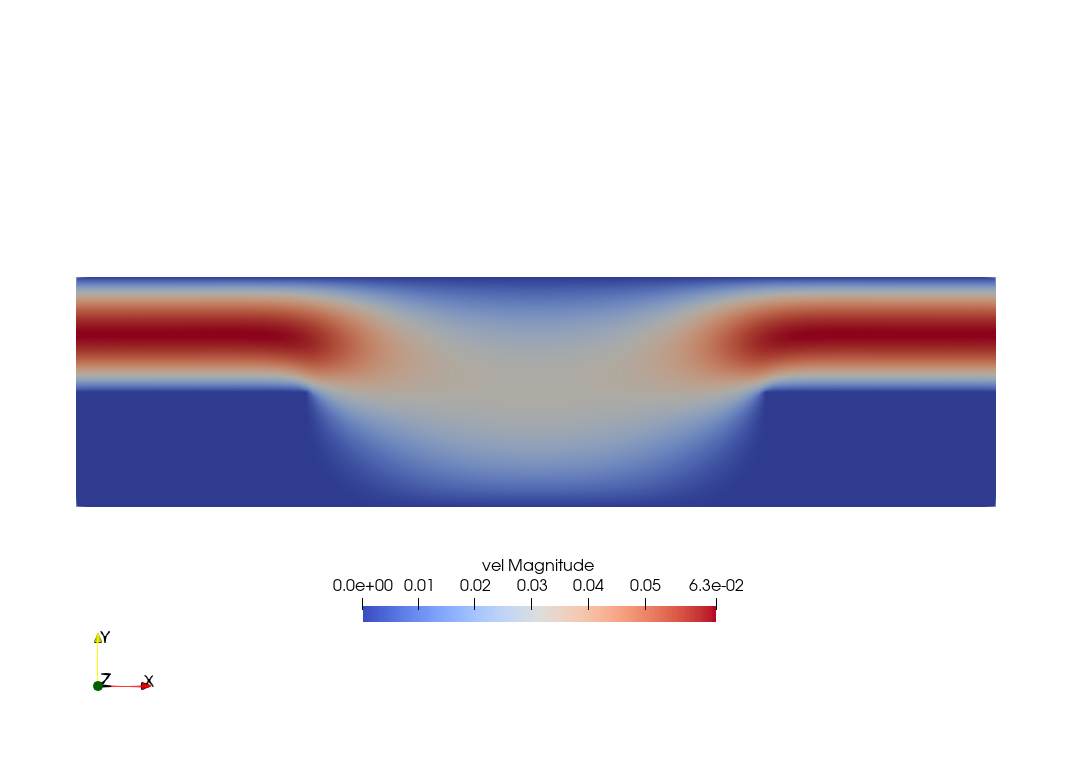
\includegraphics[width=5cm]{python_codes/fieldstone_46/results/vel}
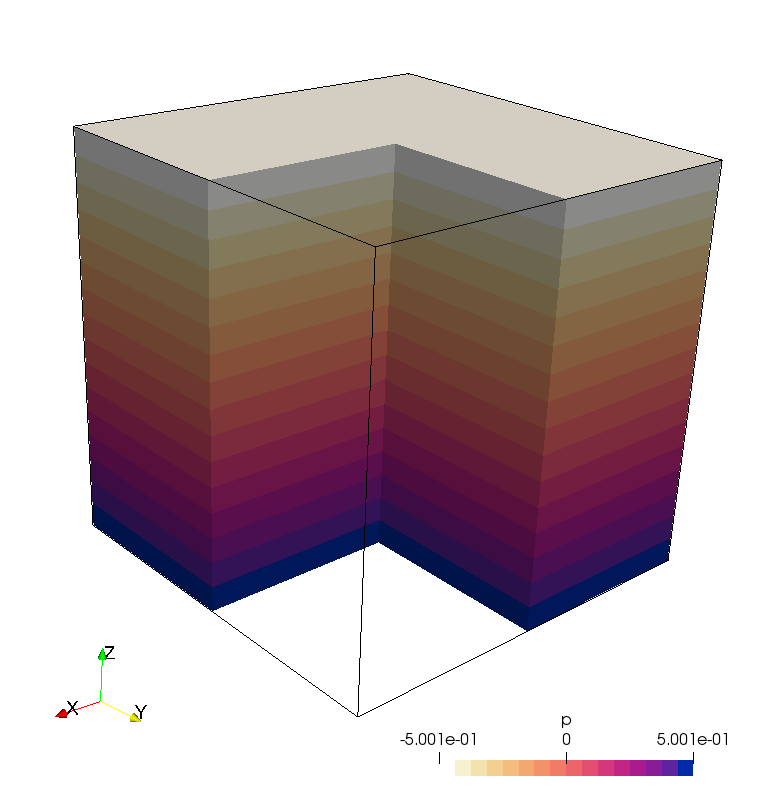
\includegraphics[width=5cm]{python_codes/fieldstone_46/results/press}\\
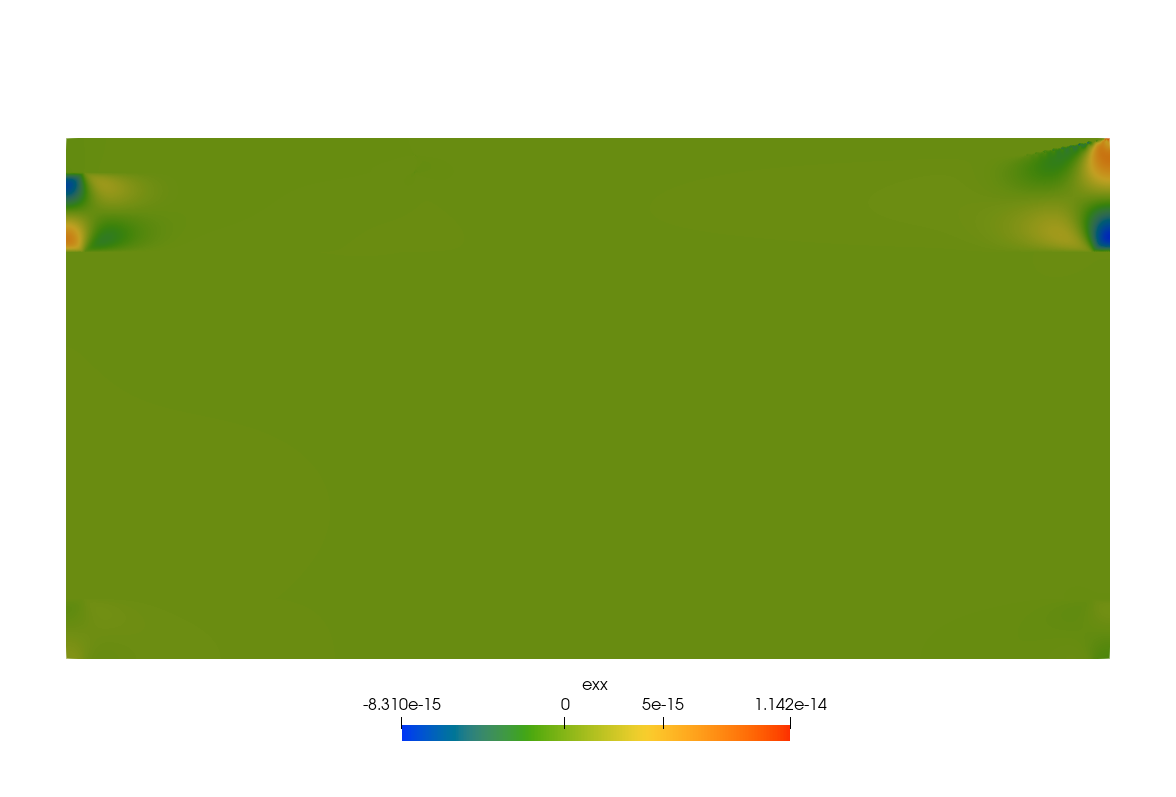
\includegraphics[width=5cm]{python_codes/fieldstone_46/results/exx}
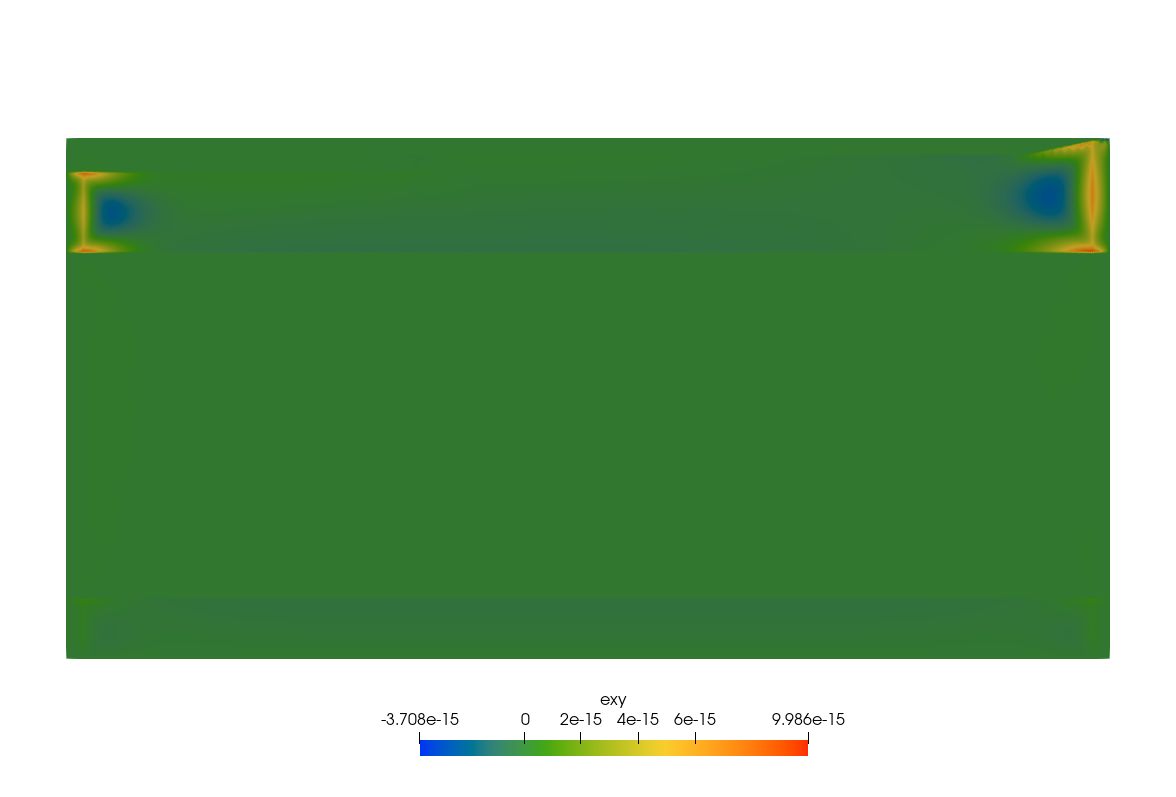
\includegraphics[width=5cm]{python_codes/fieldstone_46/results/exy}
\end{center}

\begin{center}
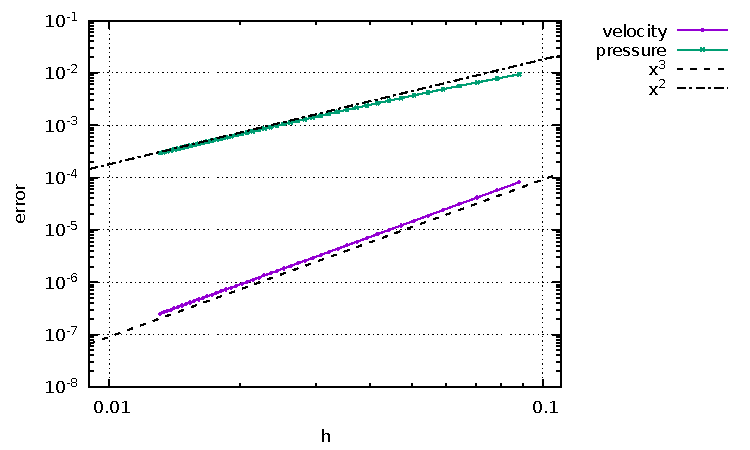
\includegraphics[width=14cm]{python_codes/fieldstone_46/results/errors.pdf}
\end{center}

